\section{Parts and Project Costs}
\label{sec:parts_and_costs}

The project costs can be broken into fixed and variable costs, where fixed costs represent the costs the team will incur during the year and production start-up costs, while variable costs represent the long-term costs associated with production.

\subsection{Fixed Costs}
\subsubsection{Prototype parts}
Through the Senior Design class, the Calvin College Engineering department provided \$750 for prototype parts. Since the project has a large scope, the team needs to minimize the cost of any single part to stay within the given budget. As such, the team chose several parts more because of their low cost rather than for functionality. As such, the team sought donations and free samples whenever possible, including the TI MSP430 development kit from Texas Instruments and the ADE7763 power monitoring chips from Analog Devices. The team also obtained a pre-purchased Xilinx Virtex-5 development board. Tables \ref{Breakers_Single.tex} through \ref{Power_Supply_Batch.tex} shows the cost of parts for Team PICA's prototype, and the cost of parts for a full scale production model. 
{
\begin{longtable}[c]{|>{\centering}b{1in}|c|c|c|>{\centering}b{1in}|c|}
\caption{Materials and Cost for a Single Breaker\label{Breakers_Single.tex}}\\
\hline
\rowcolor{blue}
Item & Quantity & Unit Price & Single System & Manufacturer Part \# & Vendor \\
\hline
\endfirsthead
\caption[]{Continued from previous page}\\

\hline
\rowcolor{blue}
Item & Quantity & Unit Price & Single System & Manufacturer Part \# & Vendor \\
\hline
\endhead
\multicolumn{6}{r}{{Continued on next page}} \\
\endfoot

\endlastfoot
Solid State Relays  & 2 & 18.42 & 36.84 & STH24D25                  & Mouser \\
\hline
5pF SMD Cap         & 2 & 0.03  & 0.06  & C0603C0G1E050C            & Mouser \\
\hline
Opto Isolator       & 2 & 3.03  & 6.06  & OPI1264C                  & Mouser \\
\hline
3.579545MHz Crystal & 1 & 0.63  & 0.63  & ABLSG-3.579545MHZ-D-2-Y-T & Mouser \\
\hline
Total:              & 7 &       & 43.59 &                           &        \\
\hline
\hline
\end{longtable}
}

{
\begin{longtable}[c]{|>{\centering}b{1in}|c|c|c|>{\centering}b{1in}|c|}
\caption{Materials and Cost for 1000 Breakers\label{Breakers_Batch.tex}}\\
\hline
\rowcolor{blue}
Item & Quantity & Price per 1000 & For 1000 Systems & Manufacturer Part \# & Vendor \\
\hline
\endfirsthead
\caption[]{Continued from previous page}\\

\hline
\rowcolor{blue}
Item & Quantity & Price per 1000 & For 1000 Systems & Manufacturer Part \# & Vendor \\
\hline
\endhead
\multicolumn{6}{r}{{Continued on next page}} \\
\endfoot

\endlastfoot
Solid State Relays  & 2    & 13.00 & 26000.00 & STH24D25                  & Mouser \\
\hline
5pF SMD Cap         & 2    & 0.005 & 10.00    & C0603C0G1E050C            & Mouser \\
\hline
Opto Isolator       & 2    & 1.76  & 3520.00  & OPI1264C                  & Mouser \\
\hline
3.579545MHz Crystal & 1    & 0.35  & 350.00   & ABLSG-3.579545MHZ-D-2-Y-T & Mouser \\
\hline
Total:              & 7.00 &       & 29880.00 &                           &        \\
\hline
\hline
\end{longtable}
}

{
\begin{longtable}[c]{|>{\centering}b{1in}|c|c|c|>{\centering}b{1in}|c|}
\caption{Materials and Cost for a Single E-Meter\label{EMeter_Single.tex}}\\
\hline
\rowcolor{blue}
Item & Quantity & Part Price & Single System & Manufacturer Part \# & Vendor \\
\hline
\endfirsthead
\caption[]{Continued from previous page}\\

\hline
\rowcolor{blue}
Item & Quantity & Part Price & Single System & Manufacturer Part \# & Vendor \\
\hline
\endhead
\multicolumn{6}{r}{{Continued on next page}} \\
\endfoot

\endlastfoot
LCD Display                     & 1   & 22.75 & 22.75  & SCLBC               & SynchroSystems \\
\hline
SSOP to DIP Adapter 20-Pin      & 2   & 3.95  & 7.90   & BOB-00499           & SparkFun       \\
\hline
Break Away Headers -- Straight  & 1   & 2.5   & 2.50   & PRT-00116           & SparkFun       \\
\hline
1N4148 Diode                    & 24  & 0.09  & 2.16   & 1N4148              & Mouser         \\
\hline
2500 Series Box Header          & 2   & 1.41  & 2.82   & N2514-6002RB        & Mouser         \\
\hline
AVE Series Electrolytic Cap 1uF & 12  & 0.07  & 0.84   & AVE105M50B12T-F     & Mouser         \\
\hline
Kehmet .033uF SMD Cap           & 12  & 0.59  & 7.08   & C1206C333KARACTU    & Mouser         \\
\hline
Kehmet .015uF SMD Cap           & 6   & 0.34  & 2.04   & C1206C153KARACTU    & Mouser         \\
\hline
Kehmet 47pF SMD Cap             & 12  & 0.07  & 0.84   & C0603C470J5GACTU    & Mouser         \\
\hline
Murata Inductor EFI             & 12  & 0.11  & 1.32   & BLM21BD102SN1D      & Mouser         \\
\hline
Maxim RS233a RS232 Driver       & 1   & 8.7   & 8.70   & MAX233CPP+G36       & Mouser         \\
\hline
D-Sub 9 Connector               & 1   & 2.32  & 2.32   & 56F404-001          & Mouser         \\
\hline
Xbee Connector 2mm pitch        & 2   & 1.6   & 3.20   & M22-7131042         & Mouser         \\
\hline
16MHz Crystal                   & 1   & 0.41  & 0.41   & ABLS-16.000MHZ-B4-T & Mouser         \\
\hline
32.768kHz Crystal               & 1   & 0.99  & 0.99   & ABS10-32.768KHZ-7-T & Mouser         \\
\hline
Tyco 6P Terminal Block          & 2   & 2.33  & 4.66   & 796949-6            & Mouser         \\
\hline
Tyco 3P Terminal Block          & 2   & 0.83  & 1.66   & 796949-3            & Mouser         \\
\hline
Varistor                        & 3   & 0.26  & 0.78   & V8ZA05P             & Mouser         \\
\hline
Current Transformer             & 3   & 6.11  & 18.33  & CST-1020            & Mouser         \\
\hline
Linear Regulator                & 3   & 1.54  & 4.62   & ZSR300GTA           & Mouser         \\
\hline
100nF SMD Cap                   & 3   & 0.7   & 2.10   & CB037D0104JBA       & Mouser         \\
\hline
22uF SMD Cap                    & 4   & 0.54  & 2.16   & EEE-1CA220SR        & Mouser         \\
\hline
18pF SMD Cap                    & 2   & 0.09  & 0.18   & CGA2B2C0G1H180J     & Mouser         \\
\hline
Red SMD LED                     & 1   & 0.4   & 0.40   & HSMC-C190           & Mouser         \\
\hline
Green SMD LED                   & 1   & 0.88  & 0.88   & HSMQ-C120           & Mouser         \\
\hline
Amber SMD LED                   & 1   & 0.4   & 0.40   & HSMA-C190           & Mouser         \\
\hline
7pF SMD Cap                     & 2   & 0.03  & 0.06   & C0603C0G1E070C      & Mouser         \\
\hline
Tact Switch                     & 2   & 0.47  & 0.94   & B3W-1052            & Mouser         \\
\hline
Total:                          & 119 &       & 103.04 &                     &                \\
\hline
\hline
\end{longtable}
}

{
\begin{longtable}[c]{|>{\centering}b{1in}|c|c|c|>{\centering}b{1in}|c|}
\caption{Materials and Cost for 1000 E-Meters\label{EMeter_Batch.tex}}\\
\hline
\rowcolor{blue}
Item & Quantity & Unit Price & Single System & Manufacturer Part \# & Vendor \\
\hline
\endfirsthead
\caption[]{Continued from previous page}\\

\hline
\rowcolor{blue}
Item & Quantity & Unit Price & Single System & Manufacturer Part \# & Vendor \\
\hline
\endhead
\multicolumn{6}{r}{{Continued on next page}} \\
\endfoot

\endlastfoot
Solid State Relays  & 2 & 18.42 & 36.84 & STH24D25                  & Mouser \\
\hline
5pF SMD Cap         & 2 & 0.03  & 0.06  & C0603C0G1E050C            & Mouser \\
\hline
Opto Isolator       & 2 & 3.03  & 6.06  & OPI1264C                  & Mouser \\
\hline
3.579545MHz Crystal & 1 & 0.63  & 0.63  & ABLSG-3.579545MHZ-D-2-Y-T & Mouser \\
\hline
Total:              & 7 &       & 43.59 &                           &        \\
\hline
\hline
\end{longtable}
}

{
\begin{longtable}[c]{|>{\centering}b{1in}|c|c|c|>{\centering}b{1in}|c|}
\caption{Materials and Cost for a Single Power Supply\label{Power_Supply_Single.tex}}\\
\hline
\rowcolor{blue}
Item & Quantity & Part Price & Single System & Manufacturer Part \# & Vendor \\
\hline
\endfirsthead
\caption[]{Continued from previous page}\\

\hline
\rowcolor{blue}
Item & Quantity & Part Price & Single System & Manufacturer Part \# & Vendor \\
\hline
\endhead
\multicolumn{6}{r}{{Continued on next page}} \\
\endfoot

\endlastfoot
1000uF Cap            & 1  & 3.18  & 3.18  & TVX1J102MCD        & Mouser  \\
\hline
10u Cap               & 3  & 0.3   & 0.90  & C1206C106K9PACTU   & Mouser  \\
\hline
100n Cap              & 2  & 0.03  & 0.06  & C1608Y5V1H104Z     & Mouser  \\
\hline
47n Cap               & 1  & 0.2   & 0.20  & C1608X7S2A473K     & Mouser  \\
\hline
2.2n Cap              & 1  & 0.16  & 0.16  & 06035C222K4Z2A     & Mouser  \\
\hline
1n Cap                & 1  & 0.03  & 0.03  & C1608X7R1H102M     & Mouser  \\
\hline
2A 30V Schottky Diode & 1  & 0.55  & 0.55  & RB060M-30TR        & Mouser  \\
\hline
4.7u Inductor         & 1  & 0.72  & 0.72  & SRR0604-4R7ML      & Mouser  \\
\hline
56K Resistor          & 1  & 1.6   & 1.60  & RG1608N-563-B-T1   & Mouser  \\
\hline
15K Resistor          & 1  & 0.1   & 0.10  & TNPW060315K0DEEA   & Mouser  \\
\hline
10K Resistor          & 1  & 1.1   & 1.10  & PAT0603E1002BST1   & Mouser  \\
\hline
1.5K Resistor         & 2  & 0.79  & 1.58  & TNPW06031K50BEEN   & Mouser  \\
\hline
10 Resistor           & 2  & 0.62  & 1.24  & TNPW060310R0BEEA   & Mouser  \\
\hline
0.1 Resistor          & 1  & 0.3   & 0.30  & CRL1206-FW-R100ELF & Mouser  \\
\hline
LM25011               & 1  & 4.86  & 4.86  & LM25011MY/NOPB     & Digikey \\
\hline
Transformer           & 1  & 23.56 & 23.56 & 166M18             & Mouser  \\
\hline
Diode                 & 4  & 0.23  & 0.92  & 1N4004G            & Mouser  \\
\hline
Total:                & 25 &       & 41.06 &                    &         \\
\hline
\hline
\end{longtable}
}

{
\begin{longtable}[c]{|>{\centering}b{1in}|c|c|c|>{\centering}b{1in}|c|}
\caption{Materials and Cost for 1000 Power Supplies\label{Power_Supply_Batch.tex}}\\
\hline
\rowcolor{blue}
Part & Quantity & Price per 1000 & For 1000 Systems & Manufacturer Part \# & Vendor \\
\hline
\endfirsthead
\caption[]{Continued from previous page}\\

\hline
\rowcolor{blue}
Part & Quantity & Price per 1000 & For 1000 Systems & Manufacturer Part \# & Vendor \\
\hline
\endhead
\multicolumn{6}{r}{{Continued on next page}} \\
\endfoot

\endlastfoot
1000uF Cap            & 1  & 2.02  & 2020     & TVX1J102MCD        & Mouser  \\
\hline
10u Cap               & 3  & 0.055 & 165      & C1206C106K9PACTU   & Mouser  \\
\hline
100n Cap              & 2  & 0.007 & 14       & C1608Y5V1H104Z     & Mouser  \\
\hline
47n Cap               & 1  & 0.036 & 36       & C1608X7S2A473K     & Mouser  \\
\hline
2.2n Cap              & 1  & 0.08  & 80       & 06035C222K4Z2A     & Mouser  \\
\hline
1n Cap                & 1  & 0.006 & 6        & C1608X7R1H102M     & Mouser  \\
\hline
2A 30V Schottky Diode & 1  & 0.169 & 169      & RB060M-30TR        & Mouser  \\
\hline
4.7u Inductor         & 1  & 0.34  & 340      & SRR0604-4R7ML      & Mouser  \\
\hline
56K Resistor          & 1  & 0.37  & 370      & RG1608N-563-B-T1   & Mouser  \\
\hline
15K Resistor          & 1  & 0.072 & 72       & TNPW060315K0DEEA   & Mouser  \\
\hline
10K Resistor          & 1  & 0.472 & 472      & PAT0603E1002BST1   & Mouser  \\
\hline
1.5K Resistor         & 2  & 0.47  & 940      & TNPW06031K50BEEN   & Mouser  \\
\hline
10 Resistor           & 2  & 0.37  & 740      & TNPW060310R0BEEA   & Mouser  \\
\hline
0.1 Resistor          & 1  & 0.121 & 121      & CRL1206-FW-R100ELF & Mouser  \\
\hline
LM25011               & 1  & 2.835 & 2835     & LM25011MY/NOPB     & Digikey \\
\hline
Transformer           & 1  & 17.28 & 17280    & 166M18             & Mouser  \\
\hline
Diode                 & 4  & 0.042 & 168      & 1N4004G            & Mouser  \\
\hline
Total:                & 25 &       & 25828.00 &                    &         \\
\hline
\hline
\end{longtable}
}

% \begin{table}[htdp]
% \caption{Prototype part costs.}
% \begin{center}
% \begin{tabular}{|c|c|c|c|c|c|}\hline\rowcolor{lightgray}
% Date & Item & Price & Quantity & Total & Running Total\\\hline
% 12-Sept & ADE7763 Samples & \$0.00 & 2 & \$0.00 & \$0.00\\\hline
% 15-Oct & SSOP to DIP Adapter 20-Pin & \$3.95 & 2 & \$7.90 & \$7.90\\\hline
% 15-Oct & Break Away Headers -- Straight	& \$2.50 & 1 & \$2.50 & \$10.40\\\hline
% 3-Nov  & TRANSF CURRENT .50" OPENING PCB & \$14.25 & 2 & \$28.50 & \$38.90\\\hline
% 15-Nov & TI Donation MSP430 & \$0.00 & 1 & \$0.00 & \$38.90\\\hline
% 02-Feb & XO Oscillators DIP-14 3.579545M & \$1.87 & 2 & \$3.74 & \$42.64 \\\hline
% 02-Feb & Solid State Relay 25A & \$24.07 & 2 & \$48.14 & \$90.78 \\\hline
% 02-Feb & LCD Graphic Display Modules & \$18.55 &1 & \$18.55 & \$109.33 \\\hline
% 02-Feb & FFC/FPC Connectors 0.5mm & \$1.29 & 2 & \$2.58 & \$111.91 \\\hline
% 02-Feb & Headers and Wire Housings & \$1.13 & 2 & \$2.26 & \$114.17 \\\hline
% 02-Feb & Synchro Chron LCD and Backlight & \$22.75 & 1 & \$22.75 & \$136.92 \\\hline
% \end{tabular}
% \end{center}
% \label{tab:proto_part_cost}
% \end{table}%

\subsection{Board Cost}
After all the dimensions were found on the parts, the Visio drawings were done in order to try to get a minimum board size to create a PCB. The PCB price was found using PCBExpress. The team did not need to pay for the PCBs originally because that service was donated by Johnson Controls Incorporated. However, if the team were to go into production they would not have this luxury. Therefore, in order to get an accurate Bill of Materials, this cost needed to be estimated at retail price along with all of the donated parts by various organizations. 

\begin{figure}[htbp]
  \centering
  \includegraphics[height=7in]{business/b_includes/Power_Supply_board_and_key}
  \caption{Power supply board mockup, 92.5 x 95 mm.}
  \label{fig:power_supply_board_mockup}
\end{figure}
\begin{figure}[htbp]
  \centering
  \subfloat[]{\label{fig:sb_board}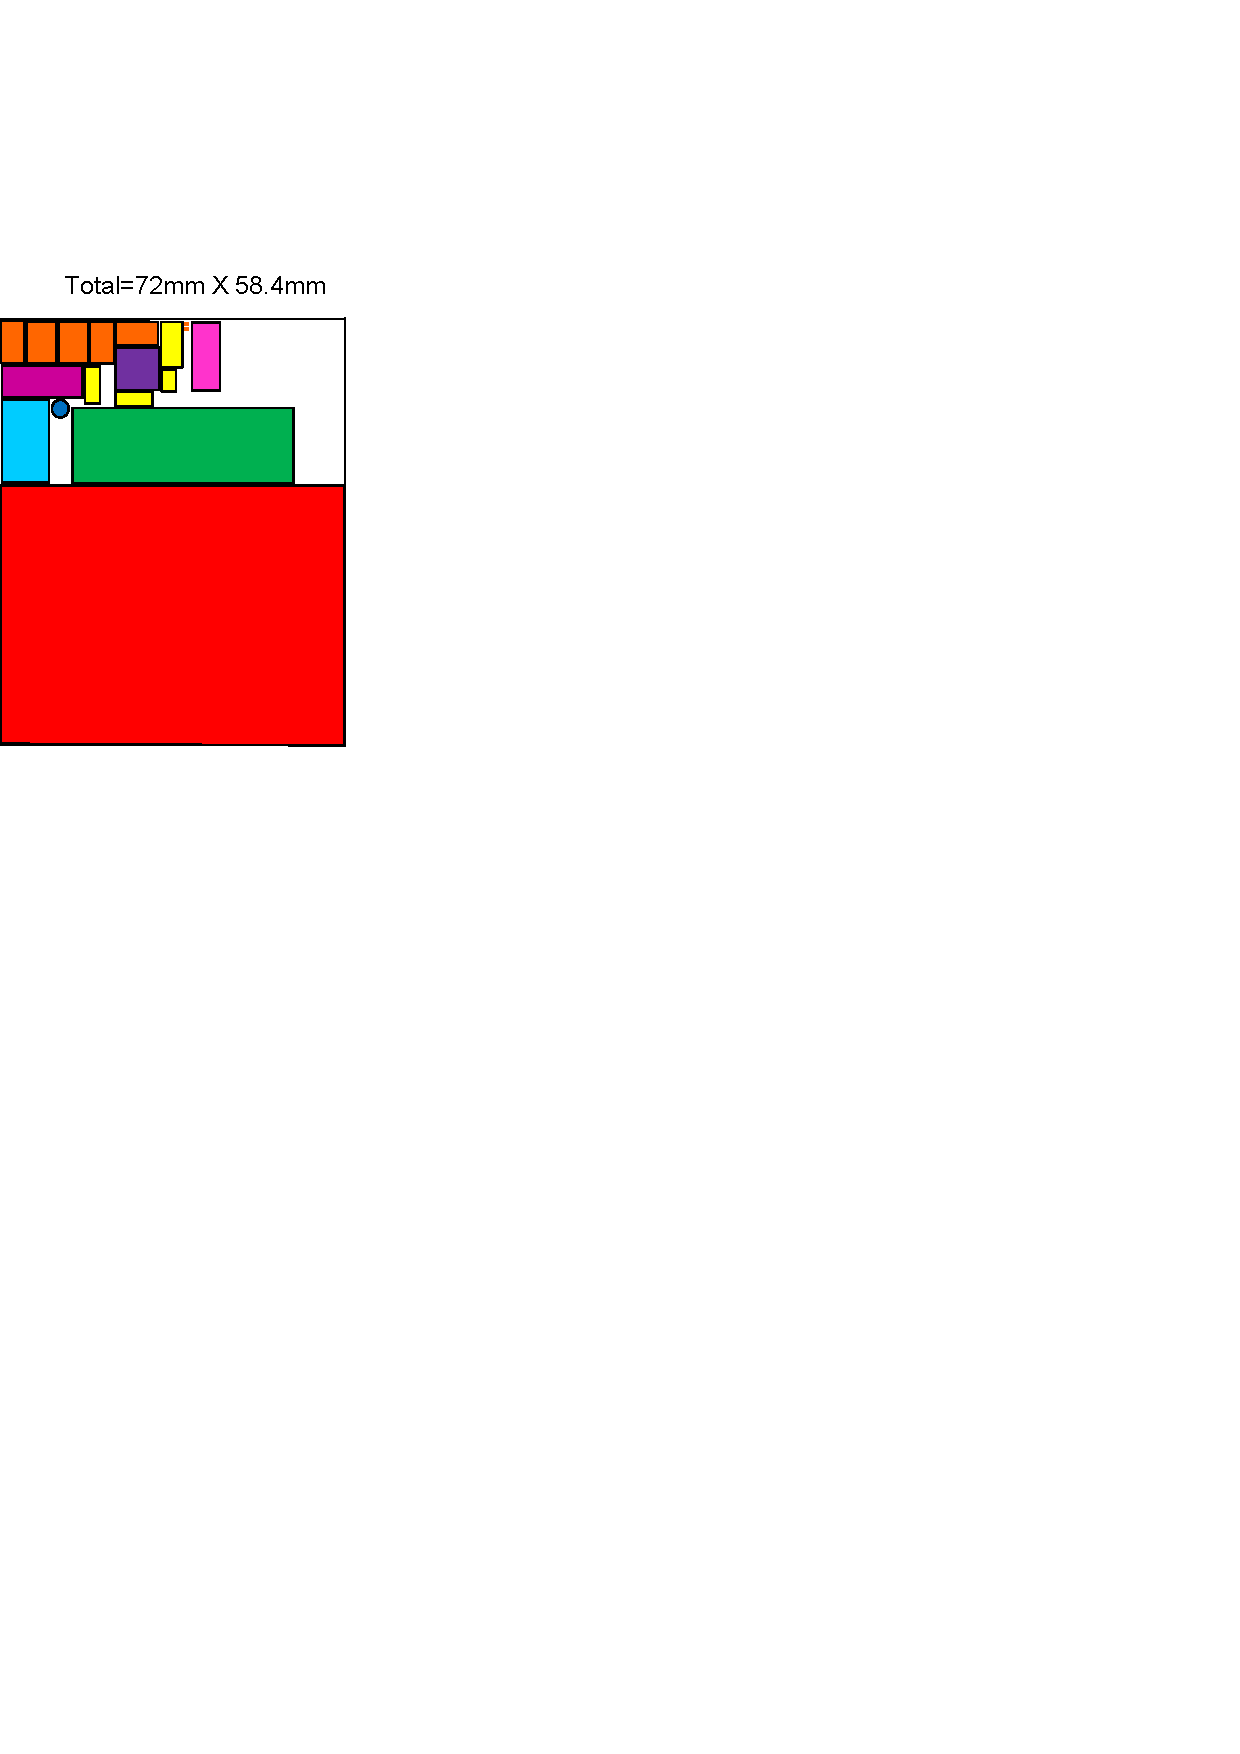
\includegraphics[width=3in]{business/b_includes/smart_breaker_board}}\\
  \subfloat[]{\label{fig:sb_key}
\includegraphics[width=2in]{business/b_includes/smart_breaker_key}}
  \caption{Smart breaker board mockup 72mm x 58.4mm.}
  \label{fig:smart_breaker_board_mockup}
\end{figure}
\begin{figure}[htbp]
  \centering
  \subfloat[]{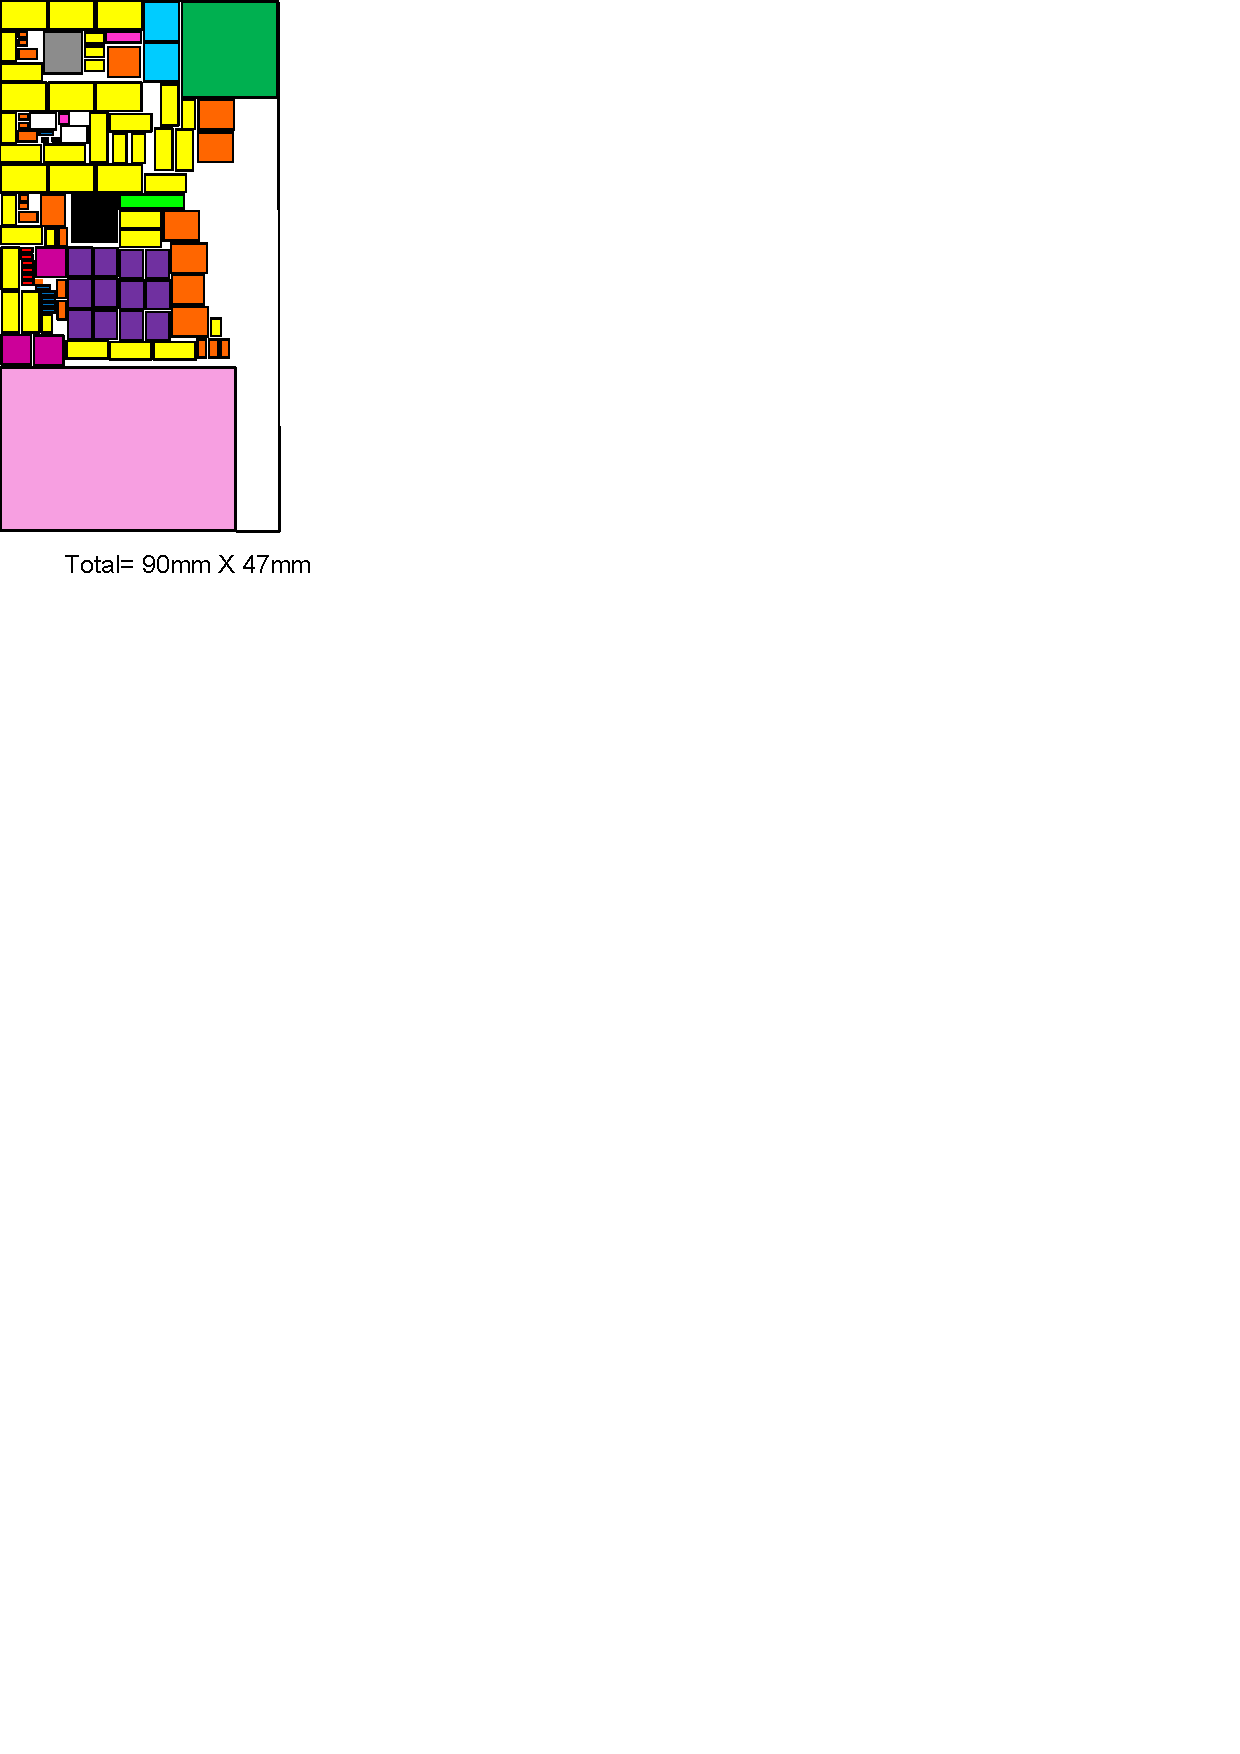
\includegraphics[height=6in]{business/b_includes/e_meter_board}}\\
  \subfloat[]{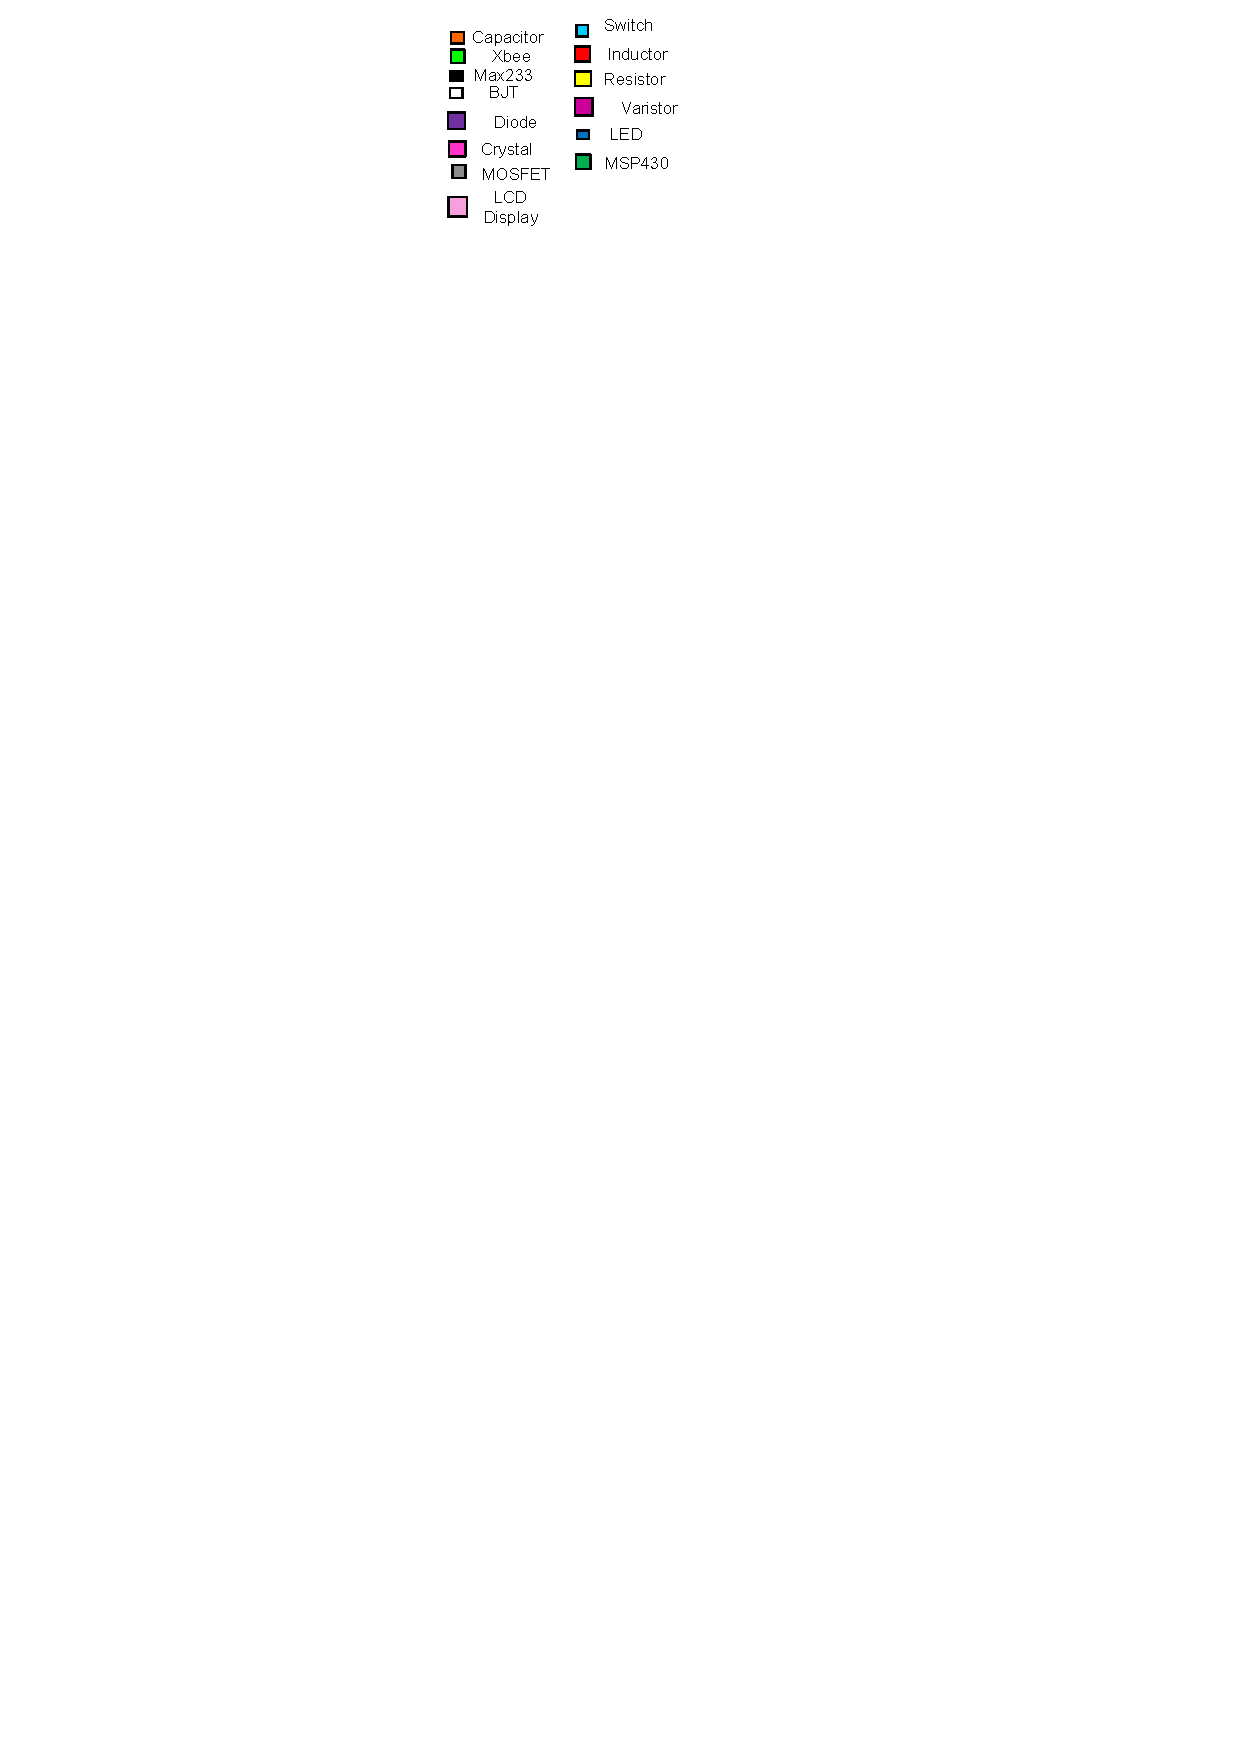
\includegraphics[width=1in]{business/b_includes/e_meter_key}}
  \caption{E-Meter board mockup 90mm x 47mm.}
  \label{fig:e_meter_board_mockup}
\end{figure}

\clearpage
\subsection{Labor}
Throughout the first and second semester, the team has kept a log of how many hours they worked. Determining the cost of labor for both semesters can accurately be assessed based on these records. For second semester so far, the team has logged 490.75 hours, with another 127.75 estimated before the end of the semester. The team also logged 388 hours for first semester, putting the yearlong total at about 1006.5 hours. Assuming engineers are paid \$100 an hour, the first semester labor cost is \$38,800, the second semester cost is \$61,850, making the full labor costs for the project \$100,650 as calculated in table \ref{tab:projecthours}. Labor has been further broken down by team member in table \ref{tab:teamprojecthours}.
\begin{table}[htbp]
  \centering
  \begin{tabular}{|c|c|c|}\hline
    \textbf{Timeframe} & \textbf{Hours Logged} & \textbf{Cost}\\\hline\hline
    First Semester     & 388                   & \$38,800\\\hline
    Second Semester    & 618.5                 & \$61,850\\\hline
    Total              & 1006.5                & \$100,650\\\hline
  \end{tabular}
  \caption{Project hours}
  \label{tab:projecthours}
\end{table}

\begin{table}[htbp]
  \centering
  \begin{tabular}{|c|c|c|c|}\hline
    Team Member      & First Semester & Second Semester & Total\\\hline\hline
    Amy Ball         & 75             & 88              & 163\\\hline
    Nathan Jen       & 107.75         & 122.75          & 230.5\\\hline
    Avery Sterk      & 95             & 209             & 304\\\hline
    Kendrick Wiersma & 125.5          & 242             & 367.5\\\hline
  \end{tabular}
  \caption{Project labor broken down by team member and semester as of 12 May 2011.}
  \label{tab:teamprojecthours}
\end{table}

\subsection{Manufacturing start-up}
In determining the cost for start-up of manufacturing, the team looked strictly at the costs of the product, ignoring many costs associated with starting a business. The team decided to contract out the work needed to build the system. Due to the high volume of systems being manufactured, the cost to manufacture will be low and is included in the cost of parts for each subsystem. The cost of constructing a storage facility is then our largest up front cost. %The team will need to determine the exact costs of this next semester, but aspects will include printing circuit boards, populating them and providing cases for each of the parts. Costs associated with buying or renting a building were broken down to a per device cost under the inventory section of the cash flow. The cost of land was determined to be irrelevant in this situation.

Table \ref{tab:labour_manufacture} shows the calculations used to determine the labor costs for manufacturing purposes. Estimates given during lecture \cite{Nielsen_Cost_Est} helped determine the hourly wage and additional costs of labor including insurance, vacation, holiday, sick time etc. The number of hours needed to assemble each system does not include the time needed to print and populate each circuit board as these will be completed by automatic machinery that requires minimal human interaction. 

\begin{table}[htdp]
\caption{Cost of labour for manufacturing}
\begin{center}
\begin{tabular}{|l|r|}\hline\rowcolor{lightgray}
Line Item & Number\\\hline
Hourly wage                                          & \$20\\\hline
Insurance, vacation, holiday, etc.	& \$10\\\hline
Per worker total	                            & \$30\\\hline
Hours to assemble breakers	         & 1\\\hline
Hours to assemble base station	& 0.5\\\hline
Hours to assemble E-meter	         & 1.5\\\hline
Breakers per year	                           &1,600,000\\\hline
Base stations per year	                  & 64,000\\\hline
E-meters per year	                           & 830,000\\\hline
Hours for breaker	                           &1,600,000\\\hline
Hours for base station	                  & 32,000\\\hline
Hours for e meter	                           & 1,245,000\\\hline
Breaker cost	                                    & \$48,000,000\\\hline
Base station Cost	                           & \$960,000\\\hline
E-meter cost	                                    & \$37,350,000\\\hline\hline
	 
Total Hours	                                    & 2,877,000\\\hline
Total Cost	                                              & \$86,310,000\\\hline
\end{tabular}
\end{center}
\label{tab:labour_manufacture}
\end{table}%

\clearpage
\subsubsection{Distribution}
The team has not yet contacted a shipping company to determine exact costs, but based on experience, size and weight, the team expects a total cost of \$25,400,000. Table \ref{tab:distribution_costs} shows the cost of distribution for each~subsystem. 

\begin{table}[htdp]
\caption{Cost of distribution}
\begin{center}
\begin{tabular}{|c|r|r|r|}\hline\rowcolor{lightgray}
	                            & Breaker	    & Base Station & E-meter\\\hline
Number shipped	& 1,600,000 & 64,000           & 830,000\\\hline
Cost per device         & \$5	     & \$12               & \$20          \\\hline
Total cost	                   & \$8,000,000   & \$768,000         & \$16,600,000\\\hline
			
Total Shipping Cost	&	\multicolumn{3}{|c|}{\$25,368,000}\\\hline
\end{tabular}
\end{center}
\label{tab:distribution_costs}
\end{table}%

%\subsubsection{Other}
%Some other costs to consider include software, discrete components, and various other development kits. In a professional engineering firm, these may represent a significant cost if they do not already own these, but as the college generously provides these, the team does not need to include them in their budget. 

\subsection{Variable Costs}
\subsubsection{Parts}
To calculate the overall cost of parts used in production, the team assumed large quantities for each of the individual components. This means that the low end of the cost range for parts is used. Based on this information and the estimated final cost of the prototype, the team calculates the cost of parts and manufacturing for the breakers, base station and e-meter to be \$35, \$100, and \$200 per subsystem, respectively.




\subsubsection{Marketing}
The project includes two distinct advertising methods to better accommodate the different target consumers. The e-meter aspect of the project will be sold directly to the power company, and the breakers and base station will be sold to the home and business owners. As the number of power companies is significantly fewer than the number of home and business owners, and will be purchasing in much larger quantities, the team decided it makes sense to appeal to the power companies in a much more personal manner. This includes phone calls, letters, and visits and outside of the cost of paying a few employees will be negligible. 

Most of the advertising will aim at the home and business owners, and the team decided that magazines and websites such as Popular Science and Green magazine are the best method of reaching out to potential buyers.  Green magazine features news and products related to sustainable energy, reaching thousands of people every year. Approximately 36\% of those people are in the building and contracting industry and would be beneficial in spreading news about the team's product \cite{GreenMediaKit}. The cost to put a medium size ad on their website is \$150 dollars per month \cite{GreenMediaKit}, so for a year would be \$1800. Popular science reaches over 7 million people using printed material. For a 1/3 page ad in four color for 12 months, the cost is \$59,900 \cite{PopSci}. The team would like to target 3 to 4 magazines and using Popular Science and Green magazine as boundary cases, estimates a total cost of \$120,000 for marketing and advertising. 

For the home and business owners' side of the project, the team also would like to work with distributers like Lowe's and Home Depot. The team would like to use a method of advertising similar to the one used for power companies, so the cost will not noticeably increase. The distribution companies may do additional advertising, but any costs associated with that will be their responsibility, so again the cost the design team expects will stay the same.

\subsubsection{Legal, warranty and support}
The team  expects about 10 hours of work for basic legal documentation. Because of the potential for lawsuits, the team built in money to cover the costs of 200 hours of work, assuming \$80 an hour, giving a total of \$16,800. The team does not intend to pursue any patents, but recognizes there may be infringement lawsuits, which were built into the above 200 hours.

The team expects 5\% of all PICA systems that include all three subsystems to fail and need replacement. At a system cost of \$260 per system with shipping of \$30, the amount needed to cover warranties is \$2,432,000.
\subsection{Total Costs}
Table \ref{ProjectCosts.tex} is a summary of the project costs, including both fixed and variable costs.

{
\small
\begin{longtable}[c]{|c|c|r|r|r|r|}
\caption{Cost estimate for the project.\label{ProjectCosts.tex}}\\
\hline
\multicolumn{5}{|>{\columncolor[gray]{0.75}}c|}{Full Scale Production} \\
\hline
\endfirsthead
\caption[]{Continued from previous page}\\

\hline
\multicolumn{5}{|>{\columncolor[gray]{0.75}}c|}{Full Scale Production} \\
\hline
\endhead
\multicolumn{5}{r}{{Continued on next page}} \\
\endfoot

\endlastfoot
\multirow{6}{*}{Fixed Costs}    & Prototyping           & \$120,700    &              &           \\\cline{2-5}
               & Automated Equipment   &    &              &                          \\\cline{2-5}
               & Marketing/Advertising & \$120,000    &              &                          \\\cline{2-5}
               & Legal        & \$168,000   &              &                          \\\cline{2-5}
               & Facilities            & \$0         &              &                          \\\cline{2-5}
               & Total                 & \$257,500   &              &                          \\\hline\hline
               
\multirow{7}{*}{Variable Costs}  & System                & Breakers  & Base station & E-meter                  \\\cline{2-5}
               & Number of devices     & 1600000   & 64000        & 830000                   \\\cline{2-5}
               & Single device parts   & 35        & 100          & 200                      \\\cline{2-5}
               & Total device parts    & 56000000  & 6400000      & 166000000               \\\cline{2-5}
               & Labor                 & \$48,000,000  & \$960,000       & \$37,350,000                 \\\cline{2-5}
               & Shipping              & \$8,000,000   & \$768,000       & \$16,600,000                 \\\cline{2-5}
               & Inventory             & \$5,100      & \$31,800        & \$6,500                     \\\cline{2-5}
               & Total (per device)& \$70        & \$127          & \$265        \\\hline\hline
\multirow{3}{*}{Totals}         & Total Per Subsystem & \$112,262,600 & \$8,417,300     & \$220,214,000                \\\cline{2-5}
               & Total per device      & \$70        & \$132          & \$265                      \\\cline{2-5}
               & Full System           & \multicolumn{3}{c|}{\$340,893,900.00}    \\\hline
\end{longtable}
}

